\section{Introduction}
%introduction of the topic
Algorithms are everywhere. They are a part of our everyday lives without even realizing it. They can be found in general mathematics, or in practical applications such as  computers or smartphones. But what exactly is an algorithm? According to the Oxford Dictionary an algorithm is generally speaken "a process or set of rules to be followed in calculations or other problem-solving operations, especially by a computer" (https://en.oxforddictionaries.com/definition/algorithm).
In our apprenticeship, we both have a lot to do with algorithms. Damian works as a software engineer, where he writes most of the time software. Stefan is an electronics engineer and his specialisation in the fourth year of education is also software. According to that, we both have a pretty good idea of what algorithms are and what they do. We found out, that each of us is fascinated by the concepts and possibilities algorithmic structures provide. So we came up with the idea, to implement an algorithm by ourselves. \bigskip
%goals
We set the goal, to program an algorithm, that can play the game Ultimate TicTacToe (UTTT). UTTT is a more complex and strategic version of the ordinary TicTacToe. 
Our approach to solve that problem is a so called Self Learning Alpha Beta Pruning Algorithm, also known as SLAP Algorithm. It's a combination of the already existing Alpha Beta Pruning algorithm combined with an own made up extension which is, as the name suggests, self learning. We want to analyse the learning process of the algorithm in more detail and evaluate whether there is really an improvement. This will be the mathematical part of our work.
To experience our algorithm in action, we also wanted to create a website where everybody can play the game against our SLAP Algorithm.
Another intention of our project is to bring the seemingly complex subject in an easy understandable form to the interested reader. We aim to resume our approach of the solution in a comprehensible way. We want to give the reader an insight and a deeper understanding of algorithms, how they work and how they are implemented. With the website, we hope to create an interesting and interactive extension to this paper.
In order to meet the requirements to cover two subjects, we decided to write our paper and the website in English. \vspace{8mm}

%overview methodological approach
The first part of our IDPA will be to implement the game itself and the corresponding SLAP algorithm. 
That includes to find a way to value the states of the game in the most efficient way. This will be the task of the evolutionary algorithm. Only if that part of the SLAP algorithm works fine, the Alpha Beta Pruning is able to work in our favour.
We decided to realise all of that with a modern programming language called Dart from Google. Dart is a well-structured, object-oriented programming language that gives us the flexibility to write client and server-side code. All with one code base and one language. Once everything is set up, we will extend our project, that we are able to track the development of the self learning part. We are also planning to integrate a function into the website where the user can train his own SLAP algorithm and observe the progress themselves.
%overview structure of the paper
%to do

\section{Rules}
To understand to game Ultimate TicTacToe, it is required to  know the rules of the ordinary TicTacToe game. If you know the rules, you can continue reading the next paragraph. 

\subsection {Rules Tic Tac Toe}
The game Tic Tac Toe consist of a 3-by-3 board. Two players are required while one player represents X and the the other player represents O. One player can start and put his mark anywhere he'd like to. After that, the other player can take his turn and put his mark to a remaining spot. This procedure continues until someone has 3 of his own marks vertically, horizontally or diagonal aligned. It's possible that no party wins and the match ends undecided.

\subsection {Rules Ultimate Tic Tac Toe}
The board of Ultimate Tic Tac Toe is made up from a 9 ordinary Tic Tac Toe boards, hence there are 81 possible fields.
Each small Tic Tac Toe board will be called a local board and the big Tic Tac Toe board will be called the global board.
A player can start anywhere he'd like to on a local board. According to the location he played on a local board, his opponent will be sent to that position in the global board. The opponent can now play on the local board, keeping in mind that he will send the other player to the relative position on the global board. 

A victory of a local board is the equivalent to a marked tile on the global board. To win the game, one has to win 3 horizontally, vertically or diagonal aligned tiles of the global board.

If a local board is won or draw, no more moves are allowed there. In case a player was sent to such a board, he is allowed to make his next turn on every other local board. It's possible that the game ends in a draw, because  no more legal moves are allowed.

\section{SLAP Algorithm}
\subsection{Alpha Beta}
Our algorithm takes a score. Each score has a certain number of moves that can be played. These are now tried out one after the other. After each move we get a new score, which also has possible moves again. Even after these moves, we have new scores again. This is how one score after the other is calculated. This can be represented as follows. Each knot (whether round or square) symbolizes a score. The branches show the possible moves. Since evaluating all scores would be too computationally intensive, a search depth is defined. In the figure the search depth would be 4, because four moves were evaluated from the main node. Now the scores of the lowest row (hands) are evaluated. The score evaluation in the graph is represented by the number in knots (do not get confused by the numbers in the other knots, more on this later). The bigger the number, the better the score for us. Now the tree is evaluated so that in the worst case the score is as high as possible for us. That means as much as assuming that the opponent always makes the move that would be worst for us. This is how the evaluation starts below. The fourth move (branches between the last two levels) is played by the opponent. Of course, this one takes the worst score for us. Therefore, the smallest number of leaves is always written in the upper node. See the example at the bottom left:
\todo{Bild aus Word kopieren oder selber erstellen}
The opponent has two moves from this score. Either he takes the first move, which leads to a score of 5, or he takes the second move, which leads to a score of 6. The first move is clearly an advantage for the opponent. Therefore, the parent node is given the value five. This happens with all nodes of this level. The third move is now played by us. We'll take the highest possible score, of course. In this way, the higher-level nodes of the previously filled level are filled with the highest of the possible values. Now it's the turn of the opponent who chooses the worst score for us. Thus, the procedure repeats itself up to the top node. In this way we get the information which train is best for us. The grey marked nodes and crossed out branches are optimizations of the algorithm. So we do not have to evaluate these areas at all and can save computing time.
\todo{Bild aus Word kopieren oder selber erstellen}
\subsection{Heuristic}
The Alpha Beta pruning decides which move is played. But it needs some information. To be more precise, you need an evaluation for each gamestat, how good it is. The better the gamestat, the higher the score. This is where the heuristic comes into play. This has only the purpose to evaluate the score.

Now to how it works. We award points for certain states. There are exactly five of these states. The check always takes place in a row, a column or a diagonal. The first two states are checked in the small fields.
\begin{itemize}
\item One field occupied, two fields empty. The condition occurs three times here. Once in the right column, once in the bottom row and once in the diagonal from top left to bottom right.
\begin{fixedpic}
	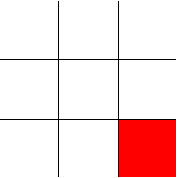
\includegraphics[width=0.33\textwidth]{con1}
	\captionof{figure}{Condition one}
\end{fixedpic}
\item Two fields occupied, one field empty. Here the condition occurs in the lowest row. Note how the first state occurs twice again, in the left and middle column.
\begin{fixedpic}
	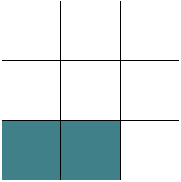
\includegraphics[width=0.33\textwidth]{con2}
	\captionof{figure}{Condition two}
\end{fixedpic}
\end{itemize}
The following three states are checked in the large field.
\begin{itemize}
\item One small field won, two small fields not yet determined. Here the condition occurs once in the top row. Here the first two states are no longer considered, a field is won a field is won.
\begin{fixedpic}
	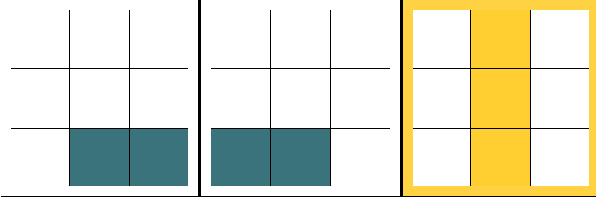
\includegraphics[width=0.33\textwidth]{con3}
	\captionof{figure}{Condition three}
\end{fixedpic}
\item Two small fields won, one small field not yet determined. Here is a visualization of this state.
\begin{fixedpic}
	\centering
	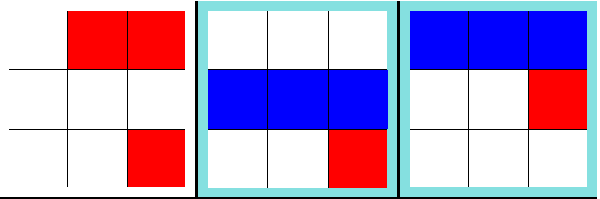
\includegraphics[width=0.6\textwidth]{con4}
	\captionof{figure}{Condition four}
\end{fixedpic}
\item Three small squares won. This also corresponds to a victory. Here the condition occurs in the right column.
\begin{fixedpic}
	\centering
	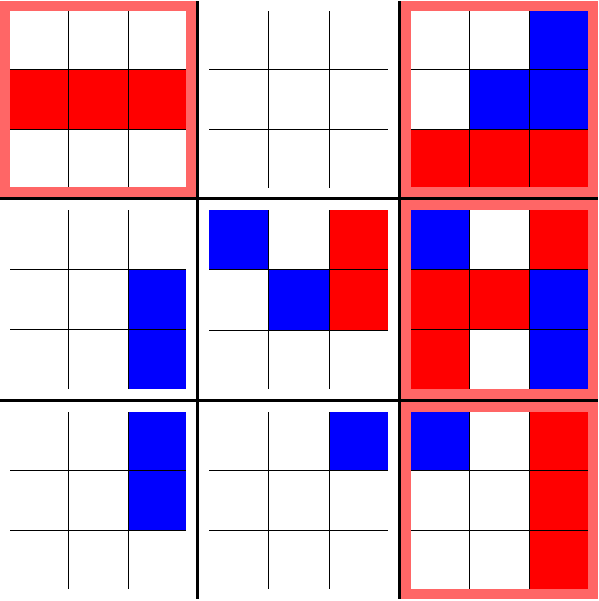
\includegraphics[width=0.6\textwidth]{con5}
	\captionof{figure}{Condition five}
\end{fixedpic}
\end{itemize}
Here I have drawn in all occurring states.
\begin{description}
\item[State one] Yellow
\item[State two] Green
\item[State three] Blue
\item[State four] Purple
\item[State five] Light blue
\end{description}
\begin{fixedpic}
	\centering
	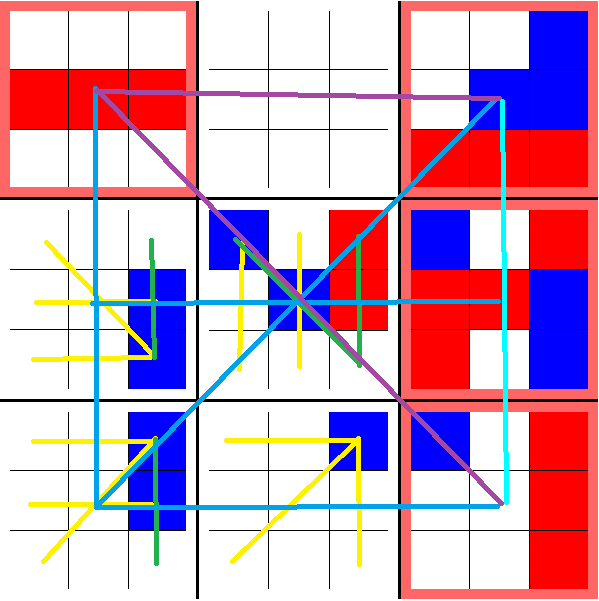
\includegraphics[width=0.6\textwidth]{allcons}
	\captionof{figure}{All Conditions}
\end{fixedpic}
The states are determined separately for both colors. Now we take the difference of the states of the two colors. Then we have a certain number for each state. Now we have to convert them into a meaningful number. This is where the DNA comes into play. The DNA is an object consisting of 5 fields. Each field stands for a factor by which the number of states is multiplied.
Let's do a sample calculation using the picture above. My DNA has the following Numbers.
\begin{description}
\item[Factor state one] 1
\item[Factor state one] 3
\item[Factor state one] 10
\item[Factor state one] 30
\item[Factor state one] 100
\end{description}
\begin{tabularx}{\textwidth}{|R|R|R|R|R|R|}
\hline
1	& 0	& 11	& -11	& 1 	& -11 \\\hline
2	& 1	& 3 	& -2	& 3 	& -6 \\\hline
3	& 4	& 0 	& 4 	& 10	& 40 \\\hline
4	& 2	& 0 	& 2 	& 30	& 60 \\\hline
5	& 1	& 0 	& 1 	& 100	& 100 \\\hline
\end{tabularx}
The effective score in this case is 183, which is all the heuristic does. Based on this information, the Alpha Beta pruning decides which move to play.







\subsection{Self Learning}



\subsection{Implementation in Dart}


\section{Progress Evaluation}

\subsection{win rate}

\section{Review}